\chapter{Jefferson Lab and CLAS12 Experimental Setup}
    \section{JLab 12 GeV CEBAF Machine}
        \subsection{Injector}
        \subsection{Accelerator and Beam Structure}
            What was the deal with looking into the time structure of the beam at JLab? Jan 2020
            Is beam polarized?
        \subsection{Other notes and comparison to CERN}
\chapter{Other Halls}
    \section{Hall A}
        \subsection{General Layout}
        \subsection{Tritium Experiment Notes}
        \subsection{BDX}
        \subsection{DVCS and DVMP Notes}
    \section{Hall C}
        \subsection{Who Cares}
    \section{Hall D}
        \subsection{Overview}
            \begin{figure}[H]
                \centering
                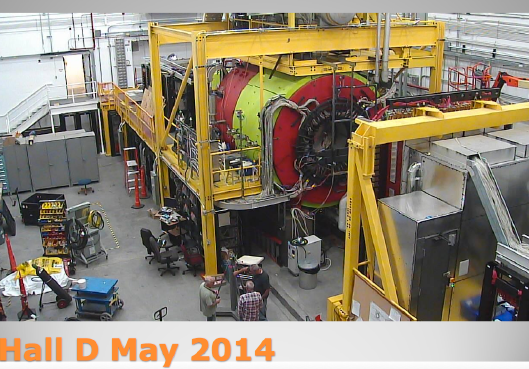
\includegraphics[width=8cm]{CLAS-12/modules/jlab/Other_Halls/HallD/Hall_Design/Hall_D.PNG}
                \caption{Hall D Overview with Solenoid}
            \end{figure}
            
            Hall D is located on the other side of the other 3 Halls at JLab and gets one extra Linac run, so is the only one able to receive the full 12 GeV beam. This hall actually uses a photon beam instead of an electron beam, as described below. The main experiments here are GlueX, PrimeX, Charged Pion Polarizability Experiment, etc.
            
        \subsection{Photon Beam Production and Structure}
            \begin{figure}[H]
                \centering
                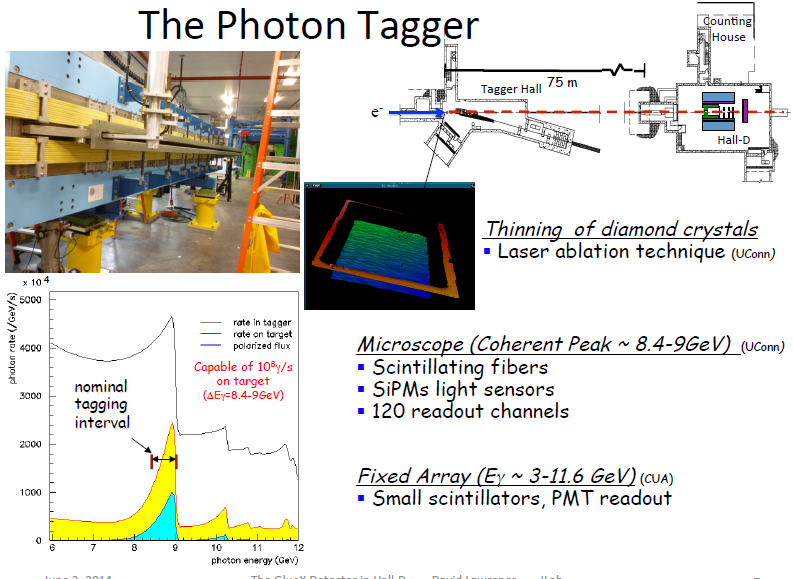
\includegraphics[width=14cm]{CLAS-12/modules/jlab/Other_Halls/HallD/Hall_Design/hall_D_Photon_tagger.PNG}
                \caption{Hall D Coherent Bremm. Photon Beam}
            \end{figure}
            
            \subsubsection{glue x pair spectrometers}
            \subsection{polarization measurement - triplet spectrometers?}
            
        \subsection{GlueX Detector Specifications}
            \begin{figure}[H]
                \centering
                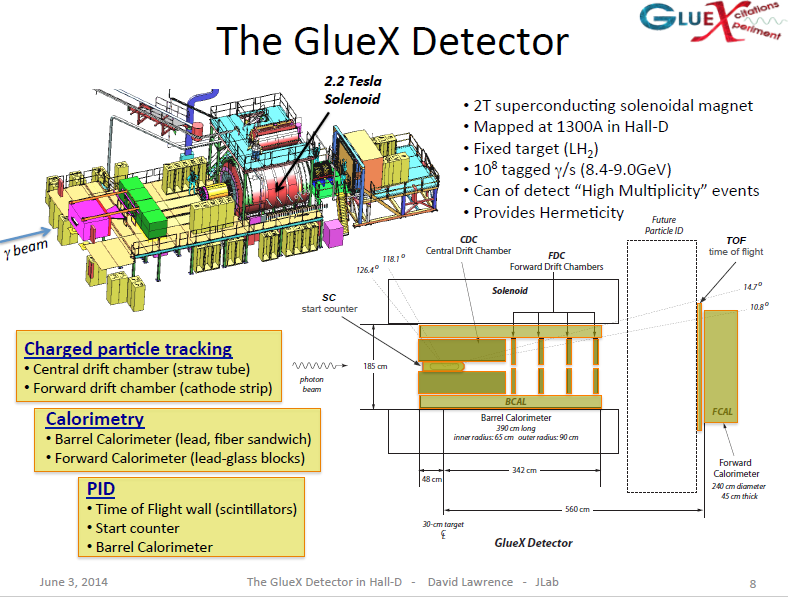
\includegraphics[width=12cm]{CLAS-12/modules/jlab/Other_Halls/HallD/Hall_Design/GlueX_Detector.PNG}
                \caption{Hall D GlueX Detector}
            \end{figure}
            
            
            CDC -  60/40 Ar/CO2 - 28 layers total - FADC 125 MHz -  resolution - $\sigma_{r\phi}$ = 150 $\mu m$
            $\sigma_{z}$ = 1.5 mm\\
            FDC - resolution 200 $\mu m$\\
            FCAL - 2800 lead glass blocks 4 x 4 x 45 $cm^3$ - PMT readout - resolution - $\frac{\sigma_E}{E} = \frac{5.7}{\sqrt{E}} + 2\%$ 
            
            \begin{figure}[H]
                \centering
                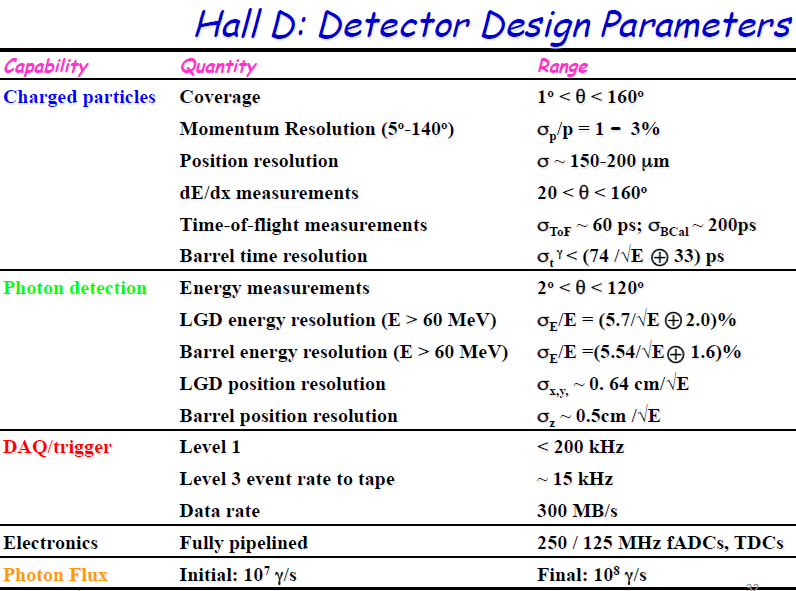
\includegraphics[width=8cm]{CLAS-12/modules/jlab/Other_Halls/HallD/Hall_Design/hall_d_design_params.PNG}
                \caption{Hall D GlueX Detector Design Specifications}
            \end{figure}
            
        \subsection{Example Experiment: Charge Pion Polarizability}
        Electric and Magnetic polarizabilities ($\alpha_{\pi}$ and $\beta_{\pi}$) are fundamental properties of particles with structure, such as the pion. In the low energy sector of QCD they can be related to the pion form factors $F_A$ and $F_V$. Leading order calculations from ChPT calculate $\alpha_{\pi}$ and $\beta_{\pi}$ to be equal in magnitude. 
        
        \begin{figure}[H]
            \centering
            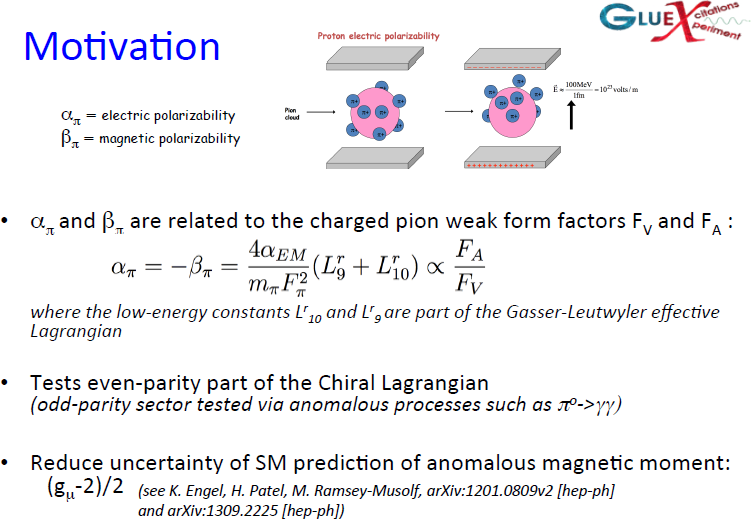
\includegraphics[width=12cm]{CLAS-12/modules/jlab/Other_Halls/HallD/cpp/cpp_motivation.PNG}
            \caption{Explanation for CPP Experiment}
        \end{figure}
            
        Experiments have been done to measure these quantities, but they do not agree with each other or ChPT:
            
        \begin{figure}[H]
            \centering
            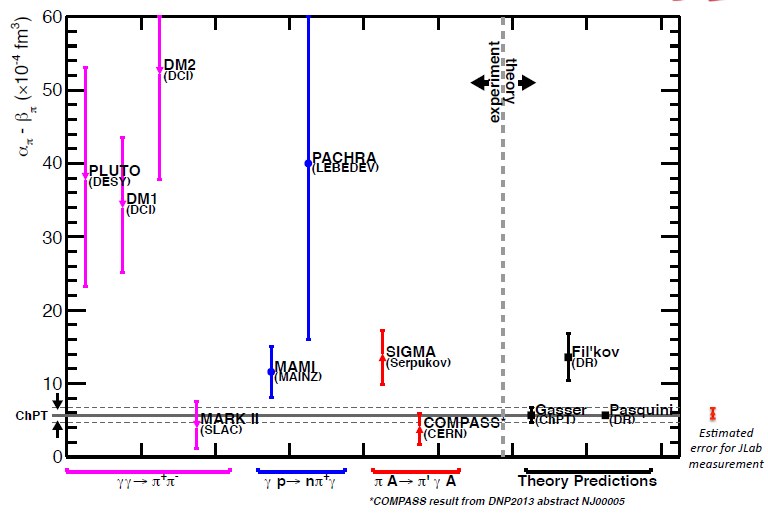
\includegraphics[width=12cm]{CLAS-12/modules/jlab/Other_Halls/HallD/cpp/cpp_motivation_plot.PNG}
            \caption{Phase Space Plot of CPP Experiments}
        \end{figure}
        
        Thus, the CPP experiment is proposed to run at glueX via the Primakoff effect ($\gamma \gamma \longrightarrow \pi \pi$. The polarizabilites will be measured as the cross section depends on these values, a factor of two difference results in a $\sim$ 10\$ diffference in cross section.
            
            \begin{figure}[H]
                \centering
                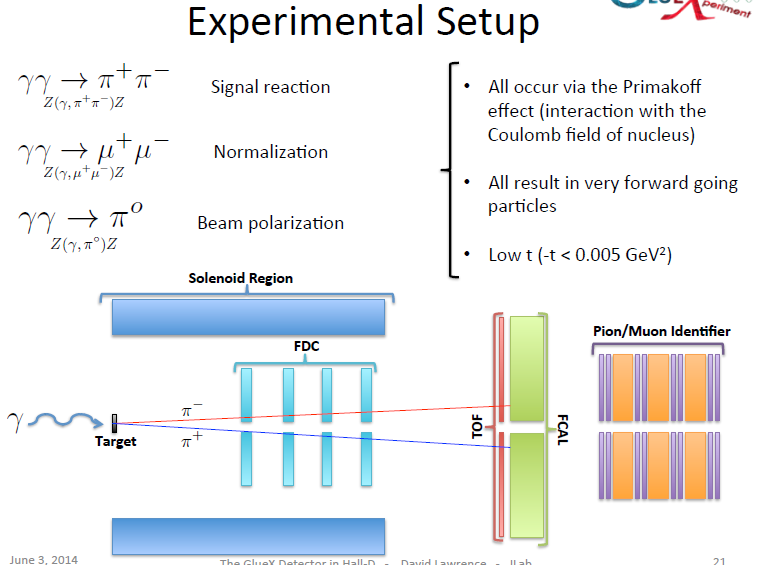
\includegraphics[width=12cm]{CLAS-12/modules/jlab/Other_Halls/HallD/cpp/cpp_experiment_setup.PNG}
                \caption{Experimental Setup for CPP Measurement}
            \end{figure}
            
            
            
            
            
            
            
\href{https://www.jlab.org/Hall-B/clas12-web/}{Detector specs here}     


            
          
          
\iffalse          
\subsection{GLUEX From Yunjie}
    I’ve heard that the oral exams this semester are all over Zoom, and pass/no record, which is nice, so you might as well just give it a shot and be done with it. I completely see what you are saying — it gets boring after a while studying it every single day! I assume you plan to do a practice sometime after you get your topic and do some reading on it? I’ll certainly tune in and provide feedback.
    
    For GlueX and/or DIRC, I agree that I don’t think they are going to be harsh about it, if they are going to ask anything at all. Nonetheless, it doesn’t hurt to know some basics. I happened to have given a student seminar talk about a year ago on GlueX+DIRC basics. I just uploaded it to the LNS students’ Oral Exam Google Drive under my personal folder, which may or may not be helpful but you can take a look.
    
    DIRC
    why it is useful to have a DIRC detector at all? I.e., why not just use a TOF or a normal cherenkov detector? 
    
    The short answer/bottom line is: GlueX physics program needs PID capabilities for K/pi separation up to 4 GeV. Our current TOF only goes up to ~ 2 GeV. We could have built a normal Cherenkov detector (i.e. it would meet our goal), but getting the BaBar DIRC is cheaper/easier(?) and does the job.
    
    Let me expand a little bit. 
    
     - Why PID? or K/pi separation for GlueX?
    The goal of the main GlueX physics program is to search for and eventually map out the hybrid meson spectrum. To do that, you need to produce and map out strange-quark-containing hybrid mesons as well. Those strange-quark-containing hybrid mesons presumably like to decay into a bunch of kaons (K+/-, K_long, K_short). People did the study and found that we need sufficient K/pi separation power (i.e. differentiating K+ from pi+, K- from pi-) up to 4 GeV.
    
    - Why not TOF?
    It cannot do the job. Our TOF timing resolution is about ~100 ps, and ~5 meters downstream of target. Actually, it’s a good exercise that they could’ve asked you during an exam to calculate the K/pi separation capability based on the timing resolution and distance. Give it a try and convince your self.
    
    - Why not a normal Cherenkov detector?
    I think we could’ve done that, but since DoE already has the DIRC bars sitting there from the decommissioned BaBar, and they studied it, and found that the DIRC can do the job and is cheaper.
    
    I assume there is some kind of advantage which makes it particulalry useful for BaBar and GlueX
    This was never formally explained to me by anyone, but I think I know the answer. For BaBar, yes, there’s a good reason: it’s very difficult to put a normal RICH type detector in the barrel region for good reasons. BaBar was a collider experiment with solenoid field design. To put RICH in the barrel region, you would need to put the whole RICH system inside, which increases the material budget and degrades the energy resolution, which is downstream. Also, PMTs don’t like magnetic fields (although you could try SiPM, but I wasn’t sure if it was available).
    
    Photon beam
    Short answer: yes, it’s probably easier to produce them in a real photon beam and also it’s easier to control the polarization of a real photon beam than that of the virtual photons in electron scattering.
    
    I think you are right that the cross section in a real photon beam is much higher. One of the most-targeted-for exotic mesons is the 1-+ state, e.g. page 9 of the slides. And photons have quantum numbers 1- -, which is a good start in that you only need to flip one quantum number, so the production cross section is likely high.
    
    Another important reason is polarization. In an electron beam, I actually don’t know how well you can control the polarization of the exchanged virtual photon, but for a real photon beam, it’s an experimental observable. Polarization is important because the silver bullet to identify those exotic mesons is their quantum numbers. To measure quantum numbers, if you can control the incoming photon beam in a polarized state, then you can basically play games like analyzing your data with different photon polarization states and show the properties of the presumably produced exotic meson follow exactly what you expect. Since I mentioned it here, I will just add something that you probably know already. If you are ever asked about things along the lines of determining quantum numbers (especially spin), it’s always good to say something along the lines of measuring the spatial/angular distributions of the decay products.
    
    I think this is likely more than enough for you to know about DIRC and GlueX. But let me know if you want to know more/anything is not clear!
    
\fi
